\documentclass{article}%
\usepackage[T1]{fontenc}%
\usepackage[utf8]{inputenc}%
\usepackage{lmodern}%
\usepackage{textcomp}%
\usepackage{lastpage}%
\usepackage[head=40pt,margin=0.5in,bottom=0.6in]{geometry}%
\usepackage{graphicx}%
%
\title{\textbf{Casado insta a "recuperar" votantes y "no dividir esfuerzos" para evitar la pérdida de escaños al Partido Popular}}%
\author{EUROPA PRESS}%
\date{04/03/2019}%
%
\begin{document}%
\normalsize%
\maketitle%
\textbf{URL: }%
http://www.eluniversal.com/internacional/34677/casado{-}insta{-}a{-}recuperar{-}votantes{-}y{-}no{-}dividir{-}esfuerzos{-}para{-}evitar{-}la{-}perdida{-}de{-}escanos{-}al\newline%
%
\textbf{Periodico: }%
EU, %
ID: %
34677, %
Seccion: %
internacional\newline%
%
\textbf{Palabras Claves: }%
NO\_TIENE\newline%
%
\textbf{Derecho: }%
2.1%
, Otros Derechos: %
\newline%
%
\textbf{\textit{"Tenemos que hacer un proyecto en el que volvamos a recuperar a aquellos que confiaron en nosotros y fueron a otras formaciones políticas, es el momento de decir que no vamos a defraudarles"}}%
\newline%
\newline%
%
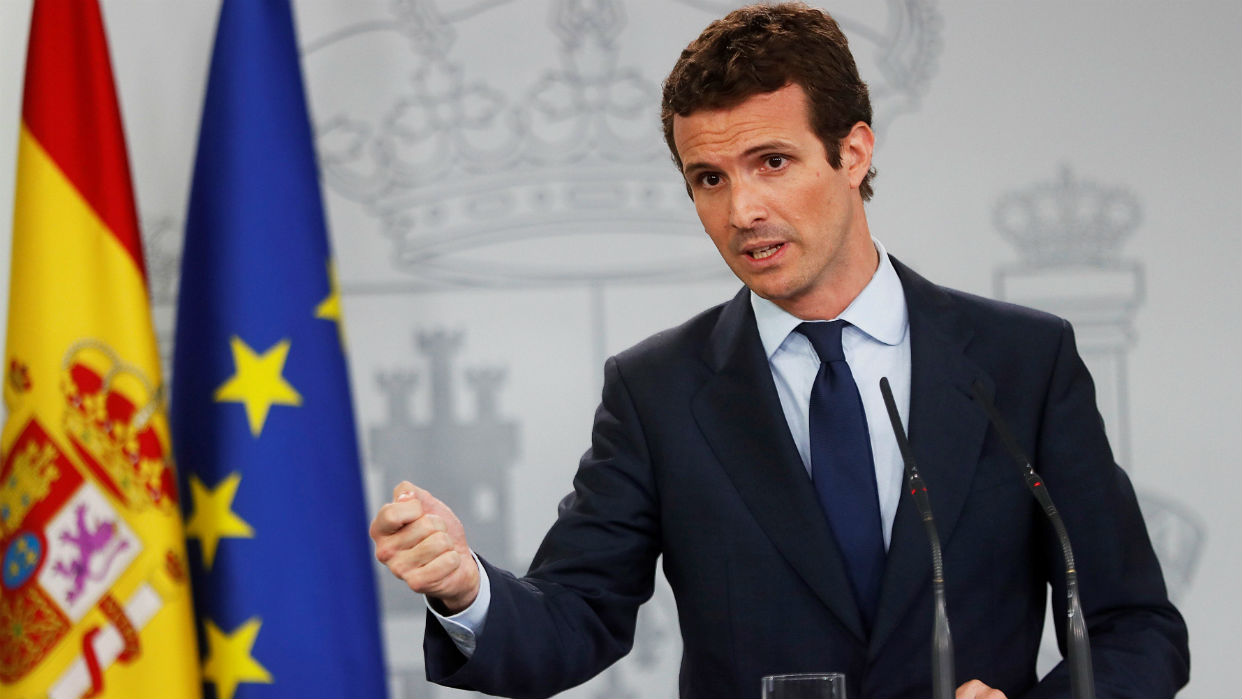
\includegraphics[width=300px]{EU_34677.jpg}%
\newline%
%
Madrid.{-}El presidente del Partido Popular de España, Pablo Casado, ha instado a "recuperar" a aquellos votantes que en su día confiaron en el PP pero que ahora%
\newline%
%
"Tenemos que hacer un proyecto en el que volvamos a recuperar a aquellos que confiaron en nosotros y que en algún momento fueron a otras formaciones políticas, es el momento de decir que este es un partido, que no vamos a defraudarles, pueden confiar en nosotros, que no dividamos esfuerzos", ha señalado Casado en la presentación de los candidatos 'populares' de la zona este de la Comunidad de Madrid, informó Europa Press.%
\newline%
%
El líder del PP pide esto porque asegura que la Ley Electoral "puede hacer que el voto a un partido determinado solo se capitalice en escaños en la mitad", es decir, "que del 100\% de votos que reciben algunas formaciones, solo el 40\% ó 50\% acaban siendo un escaño".%
\newline%
%
Además, ha hecho hincapié en la importancia de ir a las urnas para elegir a senadores 'populares', pues a su juicio "van a ser los que apliquen la Constitución en Cataluña". "Que la cruz sea para aquellos que pongan en marcha el 155", ha pedido.%
\newline%
%
\end{document}